\section{Discussion}
\subsection{Joint Laplace Noise Generation}\label{jointLap}
Recall that in \system,  both the servers, \textsf{AS} and \textsf{CSP} have to add two separate instances of Laplace noise to true answer. Thus the expected error incurred in \system is quantitatively twice that of the traditional Laplace mechanism in traditional \textsf{CDP} model. However, there is an alternative way of jointly computing a single instance of the Laplace noise via a secure multi party computation protocol~\cite{Djoin}. For this, the \CPS generates a garbled circuit that takes one $l$-bit random string from \CPS and \AS each as an input, denoted by $S_1$ and $S_2$ respectively. This circuit performs$S=S_1 xor S_2$  and uses it to generate an instance of random noise, $\eta$ drawn from the distribution $Lap(\frac{1}{\epsilon})$ following the fundamental law of transformation of probabilities.
Last, the circuit encrypts $\eta$ and returns $\boldsymbol{\eta}=labEnc_{pk}(\eta)$.
Hence, this approach adds just one instance of the Laplace noise, resulting the same accuracy guarantee as the \textsf{CDP} model. However owing to the garbled circuit, this implementation is computationally heavier. Therefore, we choose the two phase noise addition implementation for \system in this paper.
\begin{figure*}
    \begin{subfigure}[b]{0.25\linewidth}
        \centering
        %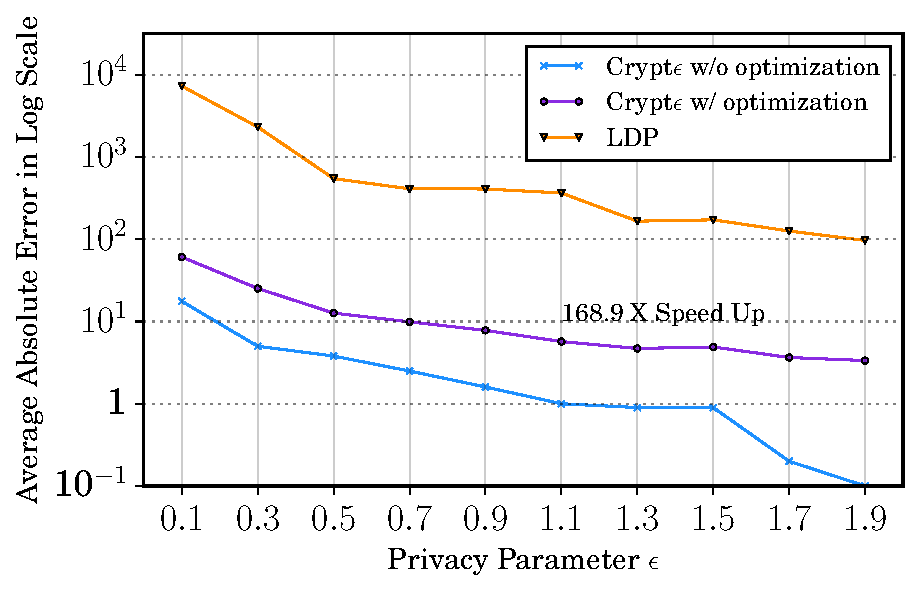
\includegraphics[width=5cm,height=3.1cm]{t1.pdf}
         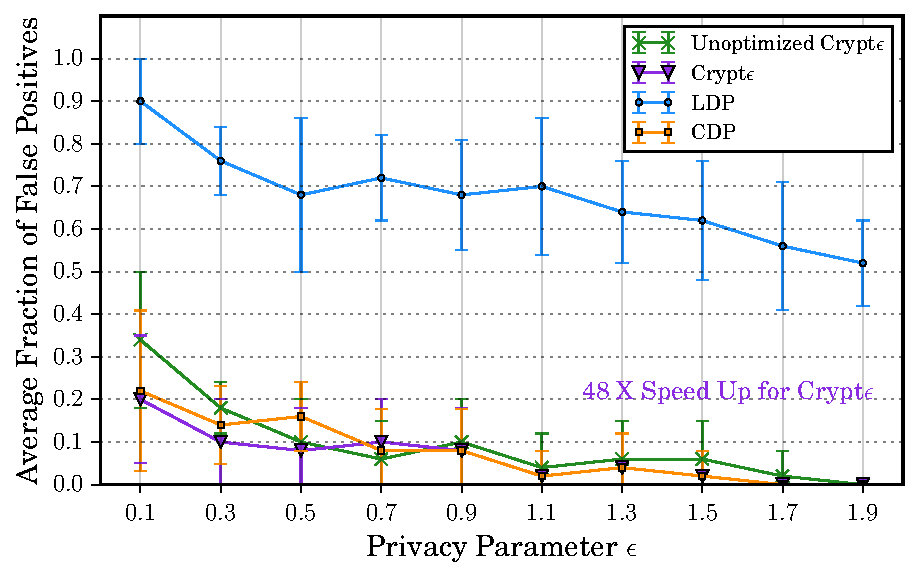
\includegraphics[width=1\linewidth]{2_final.pdf}
        \caption{ Program 2}
        \label{fig:P2}
    \end{subfigure}
    \begin{subfigure}[b]{0.25\linewidth}
    \centering 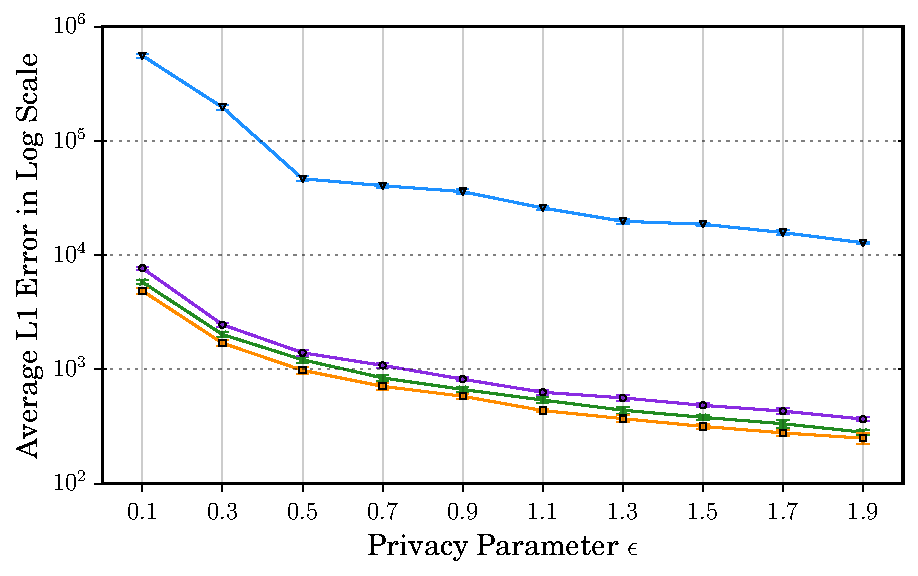
\includegraphics[width=1\linewidth]{4_final.pdf}
        \caption{Program 4}
        \label{fig:P4}\end{subfigure}
    \begin{subfigure}[b]{0.25\linewidth}
    \centering    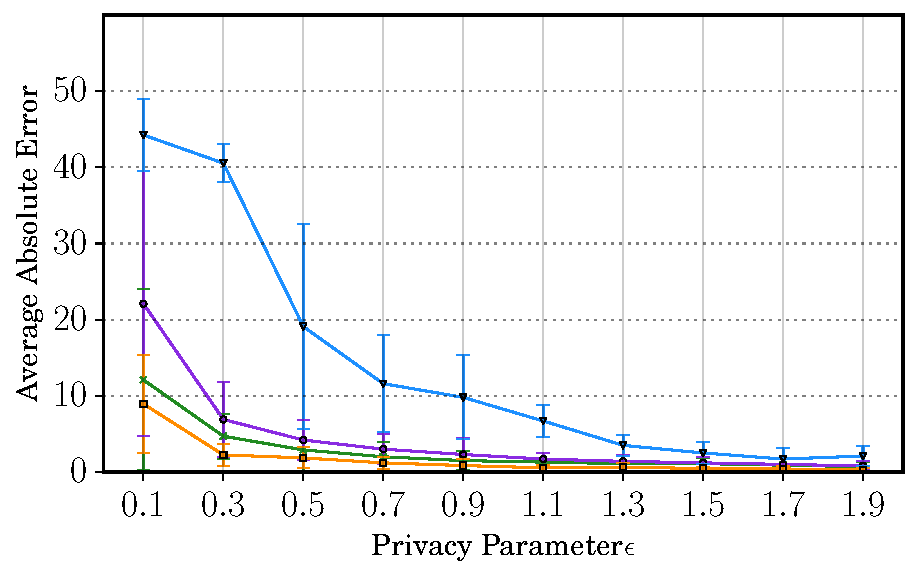
\includegraphics[width=1\linewidth]{6_finals.pdf}
        \caption{Program 6}
        \label{fig:P6}\end{subfigure}
   \caption{Accuracy Analysis of Crypt$\epsilon$ Programs Cntd.}
   \label{accuracy-appendix}
\end{figure*}

\eat{\begin{enumerate}\item takes a $l$-bit random string, $S_1$ as an input from the \textsf{CSP}
    \item takes another $l$-bit random string $S_2$ as an input from the \textsf{AS} \item performs $S=S_1 xor S_2$  and uses it to generate an instance of random noise, $\eta$ drawn from the distribution $Lap(\frac{1}{\epsilon})$ following the fundamental law of transformation of probabilities \item encrypts $\eta$ and returns $\boldsymbol{\eta}=labEnc_{pk}(\eta)$\end{enumerate}}


\subsection{Separation from LDP model}\label{app:sepldp}
As discussed in the introduction, the \textsf{LDP} model is less powerful in query answering than the \textsf{CDP} model~\cite{Kasivi,mixnets}. However, by virtue of secure computation, we can potentially implement all the functionalities of the \textsf{CDP} model in our two-server model. However, by virtue of secure computation, we can potentially implement all the functionalities of the \textsf{CDP} model in our two-server model. Functional efficiency might be a point of contention in certain cases, but nothing in the architecture of  \system can restrict its algorithmic expressibility. Recall that the power of the \textsf{LDP} model is equivalent to that of the statistical query model \cite{SQ1} from learning theory and there exists an exponential separation between the accuracy and sample complexity of local and central algorithms~\cite{Kasivi}.

We will showcase three different queries which can be computed efficiently in \system but infeasible in the standard \textsf{LDP} model.

\stitle{DNF Queries.}
The class of DNF queries fall outside the scope of statistical query models \cite{DNF}. Hence it is infeasible to answer counting queries based on a predicate with a disjunction in the \textsf{LDP} model. However, we can answer them in \system as follows.
Consider a DNF query 
$$\phi = (A_{11}\land ...\land A_{1k}) \vee ... \vee (A_{t1}\land ... A_{tl}), t, k,l \in \mathcal{Z}_{\geq 0}.$$

Let $Attribute(\phi)$ denote the set of all attributes in $\mathcal{A}$ that appear in the boolean condition $\phi$. For example, if $$\phi = \big((\mathcal{A}_1==v_1) \land \mathcal{A}_2==v_2) \vee \mathcal{A}_3==v_3 \big),$$ then we have $Attribute(\phi)=\{\mathcal{A}_1, \mathcal{A}_2,\mathcal{A}_3\}$.

Firstly, the \AS computes the attribute set $\bar{A}=Attribute(\phi)$ and projects $\encD$ on $\bar{A}$. Then, the \AS constructs the encrypted one-hot-coding of over all attributes in $\bar{A}$ using the cross product transformation. We denote the new attribute $A'$ and the new table $\encD'$. Now, the \AS simply filters this new table $\encD'$ with predicate $\phi'$  such that $\phi'$ is the equivalent of $\phi$ when expressed in terms of the new  attribute $A'$. Finally, \AS  performs the \textsf{Count} transformation and the \textsf{Laplace} transformation to obtain the final result.

\eat{
\begin{enumerate}\item Firstly, the \textsf{AS} computes the attribute set $A^*=Attribute(\phi)$.
\item Next the \textsf{AS} performs a \textsf{Project} transformation on inputs attribute set $A^*$ and the entire encrypted database $\boldsymbol{\tilde{\mathcal{D}}}$. 
\item Let $A^*= \{A^*_1,A^*_2,\ldots,A^*_t\}, t \leq k$. The \textsf{AS} constructs the encrypted one-hot-coding over the entire $t$-dimension $\lq$attribute' $\mathcal{A}^*=\times_{i=1}^t A^*_i$ by $(t-1)$ iterative application of the cross product transformation. 
\item Note that the result of the preceding step is a $m\times 1$ table where the $i^{th} , i \in [m]$ record corresponds to the encrypted one-hot-coding over the entire $t$-dimension domain space of $\mathcal{A}^*$ of data owner $\textsf{DO}_i$. Now the \textsf{AS} simply applies the \textsf{Filter} transformation on this table with predicate $\phi'$  such that $\phi'$ is the equivalent of $\phi$ when expressed in terms of the new  attribute $\mathcal{A}^*$.
\item This is followed by performing the \textsf{Count} transformation and the \textsf{Laplace} transformation to obtain the final result. 
\end{enumerate}
}

\stitle{Variable Selection Problem.} The variable selection problem is an optimization problem described as follows. Given a set of counting queries, the problem finds the query with nearly the largest value, i.e., computes an approximate argmax. Cheu et al.~\cite{mixnets} prove that the sample complexity of this problem in the "one-message" mixnet model (i.e., each user send only a single message into the shuffle) is exponentially larger than that of the \textsf{CDP} model. The variable-selection problem is actually equivalent to the exponential mechanism~\cite{Dork} in the \textsf{CDP} model. Moreover, the exponential mechanism is simply a variant of the "Report Noisy-Max" algorithm with a different noise distribution \cite{Nm}. \xh{Double check this: report noisy-max is one type of exponential mechanisms. Many exponential mechanisms are not efficient in CDP model. We do not want to over claim.} Thus essentially, the \textsf{NoisyMax} primitive in \system is capable of solving the variable-selection problem efficiently.

\stitle{Count Distinct Values.} Consider the problem of computing the number of distinct values out of a set of $m$ user data where the domain of the values is $S$ and $m<<|S|$. In the \textsf{LDP} model, for small sizes of $S$, one can construct a frequency oracle and compute the number of values with non-zero count with some careful thresholding~\cite{LDP1}. However, if the size of $S$ is huge then it becomes computationally infeasible to deploy the aforementioned mechanism. For example, if the values correspond to different URLs, since the total domain size is $2^{64}$, computation limitations make this problem infeasible to be solved in the \textsf{LDP} setting. There are mechanisms that use techniques like dividing the data into groups and then performing specialised processing etc to find top k heavy hitters in this setting \cite{HH,HH2} but still these work only for low values of $k<60$.  Although for our discussion in the paper we have considered the one-hot-coding as our preferred data encoding scheme, \system architecturally can support any arbitrary encoding scheme.  For instance, for URLs the data owners can instead use the domain name based encoding (i.e., subdomain.secondleveldomain.topleveldomain) for encrypting their data. Following this, an appropriate garbled circuit to count the number of distinct values from this encrypted dataset (which can be defined as a new Crypt$\epsilon$ primitive) can answer the above query in the \system setting.

\begin{comment}\subsection{Answering queries with disjunctions in predicate} Now let us consider a DNF query predicate $\phi=\phi_1 \vee \phi_2$ where $\phi_1=(A_1==v_1 \wedge \ldots \wedge A_n==v_n)$ and $\phi_2=(A'_1==v'_1 \wedge \ldots \wedge A'_n==v'_n)$ are two conjunctive clauses. For a given record assume, \begin{gather*}\mathbf{d}=\mathbf{c_1}\oplus \mathbf{c_2}-labMult(\mathbf{c_1,c_2}) \\
\mathbf{c_1}=genLabMult(\mathbf{\tilde{R}}_{A1}[v_1], \ldots ,\mathbf{\tilde{R}}_{An}[v_n] ) \\ \mathbf{c_1}=genLabMult(\mathbf{\tilde{R}}_{A1}[v_1], \ldots ,\mathbf{\tilde{R}}_{An}[v_n] )\end{gather*} Note that $d=1$  only iff  the record satisfies $\phi$. Thus for a two clause  DNF predicate as above, the optimized Filter transformation takes as input $x \times y$ encrypted table $\tilde{\mathbf{T}}$ with attribute set $\bigcup_{i=1}^n Attribute(\phi_i)$ and outputs a $x \times 1$ encrypted table $\mathbf{\tilde{T}}'$ such that \begin{gather} \mathbf{\tilde{T}}'[i]= \mathbf{c_1}\oplus \mathbf{c_2}-labMult(\mathbf{c_1,c_2}) \\
\mathbf{c_1}=genLabMult(\mathbf{\tilde{R}}_{A1}[v_1], \ldots ,\mathbf{\tilde{R}}_{An}[v_n] ) \\ \mathbf{c_1}=genLabMult(\mathbf{\tilde{R}}_{A1}[v_1], \ldots ,\mathbf{\tilde{R}}_{An}[v_n] )\end{gather} For $t>2$ clauses in a DNF, apply the Filter transformation pairwise for $\lceil \log t \rceil$ iterations. 
\end{comment}

An important point to be noted here is that the power of the shuffler or mixnet model  (which is obtained by augmenting \textsf{LDP} with anonymization via shuffling)~\cite{Prochlo, mixnets,amplification},  lies strictly between that of traditional \textsf{LDP} and \textsf{CDP}. Thus the two-server model of Crypt$\epsilon$ differs from this line of work in three major ways. First, \system results in no reduction in expressibility as compared to that of the \textsf{CDP} model. Second, the mixnet/shuffler model results in an approximate DP guarantee $(\epsilon\sqrt{\frac{\log\frac{1}{\delta}}{n}},\delta)$ which incurs an expected error of $O(\epsilon\sqrt{\log\frac{1}{\delta}})$.  In practice, $\delta$ has to be smaller than $\frac{1}{n}$ in order to get  meaningful privacy. In contrast, \system achieves the same order of accuracy guarantees as that of the \textsf{CDP} model. Finally, the trust assumptions of the shuffler/mixnet model differ from that of \system. Google's implementation relies on a trusted intermediary shuffler which they implement via trusted hardware enclaves. However truly secure hardware enclaves are notoriously difficult to achieve in practice \cite{Foreshadow}. The mixnet model on the other hand requires a  mix network or mixnet which is a protocol involving several computers that inputs a sequence of encrypted messages, and outputs a uniformly random permutation of those messages' plaintexts.  Their trust assumption is that at least one of the servers needs to behave honestly. For \system, both the servers are completely untrusted under the constraint that they are non-colluding and follow the protocols semi-honestly.
